\documentclass[11pt,twoside,a4paper]{article}

\usepackage{graphicx,lmodern,hyperref,calc,enumitem}
\usepackage[T1]{fontenc}
\usepackage[margin=1in]{geometry}

\begin{document}

	\title{Computing Linux Project\\
	a452}
	\author{Chris Hobbs}
	\date{May, 2015}
	\maketitle

	In this task, I will be exploring the linux commandline, and explaining the processes needed to perform some basic actions with the commandline.

	% 1
	\section{A \emph{prompt} introduction.}

		Here is the default prompt on debian linux computers:\\
		
\includegraphics{prompt}

		This prompt shows some important information to the user about the current environment that the computer is working in so that the user is able to make decisions on what to do. The prompt is made up of the following parts:

		\begin{itemize}
		    \item The current user (the part before the at-sign),
		    \item The hostname of the current computer (the part between the at-sign and the colon), and
		    \item The current directory (the part between the colon and the pound sign).
		\end{itemize}

		The current directory is shown in this example by the tilde character, which means that you are in your home directory (/home/username). The at-sign was chosen because it reflects the fact that the user is `at' the computer with the shown hostname. In the early internet, it was very likely that the user-hostname pair was actually the user's email.

	% 2
	\section{\emph{ls}ting files.}

		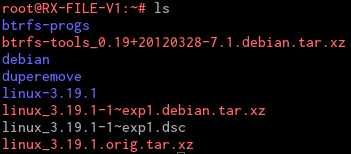
\includegraphics{ls}

		When you type \verb|ls| then press enter, you are executing the ls command. A command is simply a program which does something. They typically have short, easy to type names for convenient use at a terminal.

		The ls command in the POSIX specification (which linux conforms to), is used to list the contents - in terms of files and folders - of a directory. When used without any arguments, it lists the current directory.

		\begin{samepage}

			The output of ls is colourised, with each colour having a different meaning:\cite{ls-colours}

			\begin{description}[leftmargin=!,labelwidth=\widthof{\bfseries Light Blue}]
			    \item[Blue] directory

			    \item[White] unknown file
			    \item[Green] executable file
			    \item[Pink] image file
			    \item[Red] archive file

			    \item[Light Blue] link
			\end{description}

			In the example image above, this means that `btrfs-progs', `debian', `duperemove' and `linux-3.19.1' are directories. I'm sure you can guess the rest.

		\end{samepage}

	% 3
	\section{Playing with \emph{pipes}.}

		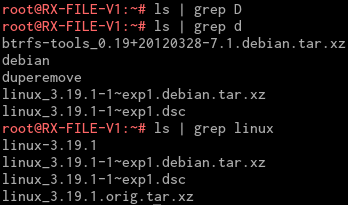
\includegraphics{ls-grep}

		The vertical bar character is used on the commandline to pipe the output of one command into the input of another. For this reason it is commonly called the pipe character. For the \verb!ls | grep D! example, we are piping the output of \verb|ls| (a listing of the current directory) into the \verb|grep| command, which searches each line of output from ls (in this case a file/directory name) for the character `D'. This means that the output shows a list of files and directories whose names contain a capital D. Because none of the files in the home directory of my linux computer have a `D' character in them, I tried grep again with a lowercase `d', and got a result. I also tried grepping for `linux' which returned a list of files containing the word linux.

	% 4
	\section{\emph{Redirecting} all the things.}

		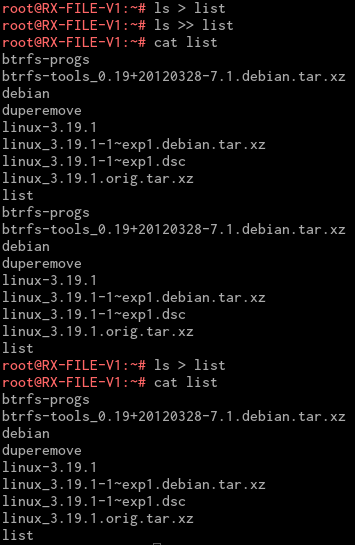
\includegraphics{redirection}

		In linux commandlines, \verb|>| is used to redirect the output of a command - like pipes - but to a file instead of another command.\cite{lts-redirection} At first, it doesn't look like \verb|>| and \verb|>>| do anything at all, but I found out what they do using the internet. I also found out that \verb|>| overwrites the contents of the file it is writing to while \verb|>>| appends the contents of the output to the bottom of the file. In the example I list above, I use the \verb|cat| command to print the contents of the `list' file that I have created by output redirecton. You can see the contents of \verb|ls| printed twice the first time because I had used \verb|>>| to append the contents of the file when it already had the contents once. Using \verb|ls > list| replaces the contents of the file with the output of \verb|ls| therefore the last \verb|cat| only prints the output of ls once.

	% 5
	\section{\emph{cd} aw\textsuperscript{aa\textsuperscript{a\textsuperscript{a\textsuperscript{\textsuperscript{y}}}}}}

		The \verb|cd| (\emph{c}hange \emph{d}irectory) command is used to change the current directory. \empth|..| is a shortcut in linux for the parent directory of the current one. For example if you are in the directory \verb|/home/chris/|, \verb|..| would be \verb|/home/|. In my example, where the current directory is \verb|/root/| (the home directory of the root user), using \verb|cd ..| would take me to the root directory. We can verify this with the \verb|pwd| command.\cite{lts-navigation}

		The second command (\verb|cd /etc|) - unlike the first - uses a absolute directory name instead of a relative one. Absolute directory names always begin with a \verb|/| because they are specifying the whole path to get to the directory, which always starts from the root of the file system, just like an absolute path always begins with the drive letter on windows.

		The third command is much like the second, except it takes you to the root of the filesystem in linux.

		The fourth command (\verb|cd ~|) uses a shortcut simililar to \verb|..| to take you to your home directory. In linux \verb|~| is always the path to that user's home directory. You can also use \verb|~username| to take you to any user's home directory. For example \verb|~chris| would take you to the home directory of the user `chris'.

	% 6
	\section{\emph{mk}ing \emph{dir}ectories}

		The \verb|mkdir| command is used to make a directory (REF)

	% end page
	\newpage
	\begin{thebibliography}{9}

		\bibitem{ls-colours}
			karthick87,
			\emph{What do the different colors mean in the terminal?},
			Ask Ubuntu,
			http://askubuntu.com/a/17300

		\bibitem{lts-redirection}
			William E. Shotts, Jr.,
			\emph{Learning the shell - Lesson 7: I/O Redirection},
			LinuxCommand.org,
			http://linuxcommand.org/lc3\_lts0070.php

		\bibitem{lts-navigation}
			William E. Shotts, Jr.,
			\emph{Learning the shell - Lesson 2: Navigation}
			LinuxCommand.org,
			http://linuxcommand.org/lc3_lts0020.php
		

	\end{thebibliography}

	\vfill
	This document was typed up using \LaTeX. Which is why it looks so professional. Hey look examiner, I'm learning yet \emph{more} life skills!

\end{document}
